% !TeX program = xelatex
% !TeX root = representation_final.tex
% !TeX encoding = UTF-8
% !TeX spellcheck = en_US
% arara: xelatex: { interaction: nonstopmode, synctex: yes }
% arara: xelatex: { interaction: nonstopmode, synctex: yes }
%
% Auto-build note:
% - VS Code LaTeX Workshop: enable "latex-workshop.latex.autoBuild.run": "onSave".
% - TeXstudio/TeXShop can use the magic comments above to choose XeLaTeX.
% - Manual command from final_submission/:
%   bash watch_representation_final.sh
% - Automatic watch (save-to-recompile):
%   bash watch_representation_final.sh representation_final.tex

\documentclass[aspectratio=169,10pt]{beamer}

\usepackage{fontspec}
\usepackage{graphicx}
\usepackage{booktabs}
\usepackage{array}
\usepackage{tabularx}
\usepackage{amsmath,amssymb}
\usepackage{xcolor}
\usepackage{tikz}
\usetikzlibrary{arrows.meta,positioning,calc}

\graphicspath{{figures/}}

% Fudan-inspired, projector-safe palette.
\definecolor{fudanblue}{HTML}{0B4EA2}
\definecolor{fudanmid}{HTML}{2F68B2}
\definecolor{fudanlight}{HTML}{EEF4FC}
\definecolor{textgray}{HTML}{333333}
\definecolor{mutedgray}{HTML}{6B7280}
\definecolor{rulegray}{HTML}{D7DCE5}
\definecolor{accentorange}{HTML}{D97904}
\definecolor{accentgreen}{HTML}{008A5B}

\newcommand{\pos}[1]{\textcolor{fudanblue}{#1}}
\newcommand{\warn}[1]{\textcolor{accentorange}{#1}}
\newcommand{\HL}[1]{\textcolor{accentgreen}{#1}}

\setbeamertemplate{navigation symbols}{}
\setbeamersize{text margin left=0.72cm,text margin right=0.72cm}
\setbeamercolor{normal text}{fg=textgray,bg=white}
\setbeamercolor{frametitle}{fg=fudanblue,bg=white}
\setbeamercolor{item}{fg=fudanblue}
\setbeamercolor{caption name}{fg=fudanblue}
\setbeamerfont{frametitle}{series=\bfseries,size=\Large}
\setbeamerfont{framesubtitle}{size=\small}
\setbeamerfont{title}{series=\bfseries,size=\LARGE}
\setbeamerfont{subtitle}{size=\large}
\setbeamerfont{itemize/enumerate body}{size=\small}
\setbeamerfont{itemize/enumerate subbody}{size=\small}

\setbeamertemplate{itemize item}{\color{fudanblue}\scriptsize$\blacksquare$}
\setbeamertemplate{itemize subitem}{\color{fudanblue}\scriptsize$\blacktriangleright$}

\newcommand{\maybelogo}[2]{%
  \IfFileExists{figures/#1}{\includegraphics[#2]{#1}}{}%
}

\newcommand{\fig}[2][]{%
  \IfFileExists{figures/#2}{\includegraphics[#1]{#2}}{%
    \fbox{\begin{minipage}[c][0.34\textheight][c]{0.94\linewidth}
      \centering\small Missing figure:\\ \texttt{\detokenize{figures/#2}}
    \end{minipage}}%
  }%
}

\newcommand{\keyline}[1]{%
  \vspace{0.04cm}
  \noindent\begin{tabular}{@{}m{2.2pt}@{\hspace{0.55em}}m{0.90\linewidth}@{}}
    {\color{accentgreen}\rule{2.2pt}{1.35em}} & \textbf{#1}
  \end{tabular}
  \vspace{0.09cm}
}

\newcommand{\metric}[2]{%
  \begin{minipage}[t]{0.30\linewidth}
    \centering
    {\Large\bfseries\color{fudanblue}#1}\\[-1pt]
    {\scriptsize\color{mutedgray}#2}
  \end{minipage}
}

\newcommand{\smallnote}[1]{%
  {\scriptsize\color{mutedgray}#1}
}

\setbeamertemplate{frametitle}{%
  \begin{tikzpicture}[remember picture,overlay]
    \node[anchor=north west,inner sep=0pt] at ($(current page.north west)+(0.78cm,0cm)$)
      {\maybelogo{fudan_logo.png}{height=1.34cm}};
    \node[anchor=north west,align=left,text width=0.74\paperwidth] at ($(current page.north west)+(2.58cm,-0.47cm)$)
      {{\usebeamerfont{frametitle}\color{fudanblue}\insertframetitle\par}
       {\usebeamerfont{framesubtitle}\color{fudanblue!72!black}\insertframesubtitle\par}};
  \end{tikzpicture}
  \vspace{1.42cm}
}

\setbeamertemplate{footline}{%
  \leavevmode
  \hbox{\hspace{0.72cm}\scriptsize\color{mutedgray}\insertframenumber/\inserttotalframenumber}
  \vspace{0.20cm}
}

\title{CNN Representation-Assisted MMMD}
\subtitle{From Power Improvement to Biomedical Domain-Shift Interpretation}
\author{Individual Component}
\date{June 2026}


\begin{document}

{% title page
\begin{frame}[plain]
  \begin{tikzpicture}[remember picture,overlay]
    \fill[white] (current page.south west) rectangle (current page.north east);
    \begin{scope}
      \clip ($(current page.south east)+(-5.85cm,0cm)$) --
            ($(current page.north east)+(-2.62cm,0cm)$) --
            (current page.north east) --
            (current page.south east) -- cycle;
      \IfFileExists{figures/fudan_background.png}{%
        \node[anchor=south east,inner sep=0pt] at (current page.south east)
          {
\includegraphics[width=0.68\paperwidth,height=\paperheight]{fudan_background.png}};
      }{%
        \fill[fudanblue] (current page.south west) rectangle (current page.north east);
      }
    \end{scope}
    \node[anchor=north west,inner sep=0pt] at ($(current page.north west)+(0.78cm,0cm)$)
      {\maybelogo{fudan_logo.png}{height=1.75cm}};
    \node[anchor=north west,inner sep=0pt] at ($(current page.north west)+(0.88cm,-2.58cm)$) {%
      \begin{minipage}{0.60\paperwidth}
        \raggedright
        {\color{textgray}\usebeamerfont{title}\inserttitle\par}
        \vspace{0.20cm}
        {\color{textgray}\usebeamerfont{subtitle}\insertsubtitle\par}
        \vspace{0.58cm}
        {\color{textgray}\large\insertauthor\par}
        \vspace{0.12cm}
        {\color{textgray}\insertdate\par}
      \end{minipage}
    };
  \end{tikzpicture}
\end{frame}
}


% -------------------------------------------------------------------
\begin{frame}{Foundation-Encoder Component}{A two-axis extension of the CNN-MMMD experiments}
\keyline{Keep the two-sample test fixed where possible, and vary the image representation explicitly.}
\vspace{0.20cm}
\begin{columns}[T,totalwidth=\linewidth]
\begin{column}{0.48\linewidth}
\textbf{\pos{Axis 1: image representation}}
\begin{itemize}
  \item Raw pixels: direct baseline for image-space MMMD.
  \item CLIP: frozen image-language foundation encoder.
  \item DINOv2: frozen self-supervised visual encoder.
  \item CNN: task-trained feature extractor from the reproduction pipeline.
\end{itemize}
\end{column}
\begin{column}{0.48\linewidth}
\textbf{\HL{Axis 2: testing layer}}
\begin{itemize}
  \item Original paper: Gaussian multi-kernel MMMD, mainly GAUSS5/GEXP-5.
  \item Our extension: NEW-MMMD with covariance stabilization and kernel pruning.
  \item Metrics: power, Type-I error, and sample-size efficiency.
\end{itemize}
\end{column}
\end{columns}
\end{frame}

% -------------------------------------------------------------------
\begin{frame}{Datasets Used in the Foundation-Encoder Experiments}{Local biomedical image datasets and mixture tasks}
\begin{columns}[T,totalwidth=\linewidth]
\begin{column}{0.60\linewidth}
  \fig[width=\linewidth,height=0.58\textheight,keepaspectratio]{foundation_dataset_examples.png}
\end{column}
\begin{column}{0.36\linewidth}
  \scriptsize
  \textbf{\pos{BloodMNIST-224}}\\
  17,092 blood-cell images. Main task: $(0,1,3)$ vs $(0,1,6)$ under six noise levels.

  \vspace{0.45em}
  \textbf{\pos{PathMNIST-28}}\\
  107,180 pathology patches. Used for the dechao-aligned mixture comparison.

  \vspace{0.45em}
  \textbf{\pos{NCT-CRC}}\\
  100,000 H\&E patches. Main task: $(\mathrm{NORM,STR,LYM})$ vs $(\mathrm{TUM,STR,LYM})$.

  \vspace{0.60em}
  \textbf{Roles in this section}
  \begin{itemize}
    \item BloodMNIST: noise robustness.
    \item PathMNIST: CNN comparison.
    \item NCT-CRC: sample size and NEW-MMMD.
  \end{itemize}
\end{column}
\end{columns}
\end{frame}

% -------------------------------------------------------------------
\begin{frame}{CLIP and DINOv2}{Frozen visual foundation encoders used as image representations}
\begin{columns}[T,totalwidth=\linewidth]
\begin{column}{0.48\linewidth}
\textbf{\pos{CLIP image encoder}}
\begin{itemize}
  \item Trained with image--text contrastive learning on large-scale web data.
  \item Produces a compact image embedding aligned with language-level semantics.
  \item Useful as a broad zero-shot representation, but may under-emphasize fine biomedical morphology.
  \item In this project: images are resized/preprocessed, then encoded once and cached.
\end{itemize}
\end{column}
\begin{column}{0.48\linewidth}
\textbf{\HL{DINOv2 visual encoder}}
\begin{itemize}
  \item Self-supervised vision transformer trained to learn visual structure without labels.
  \item Produces morphology-sensitive features that are often strong for pathology-style images.
  \item Does not use dataset labels during feature extraction, so it is a frozen representation baseline.
  \item In this project: DINOv2 embeddings are compared with CLIP, raw pixels, and trained CNN features.
\end{itemize}
\end{column}
\end{columns}

\vspace{0.22cm}
\begin{center}
\smallnote{Both encoders are used only as feature extractors; the two-sample testing step is still performed by MMMD-style methods.}
\end{center}
\end{frame}

% -------------------------------------------------------------------
\begin{frame}{Experiment Map}{Separate three representation studies from one testing-layer study}
\begin{center}
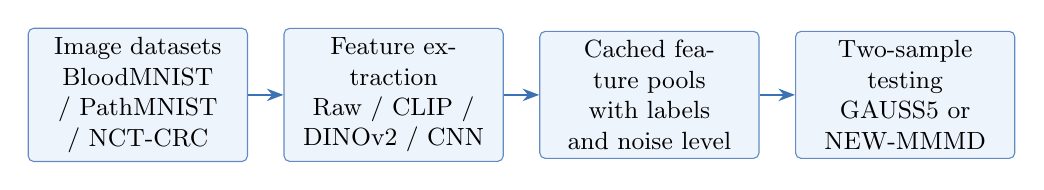
\begin{tikzpicture}[
  node distance=0.45cm,
  flowbox/.style={draw=fudanblue!65, fill=fudanlight, rounded corners=2pt,
                  minimum height=0.78cm, text width=2.55cm, align=center, font=\small},
  arr/.style={-{Stealth[length=2.1mm]}, thick, draw=fudanblue!80}
]
  \node[flowbox] (data) {Image datasets\\BloodMNIST / PathMNIST / NCT-CRC};
  \node[flowbox, right=of data] (repr) {Feature extraction\\Raw / CLIP / DINOv2 / CNN};
  \node[flowbox, right=of repr] (pool) {Cached feature pools\\with labels and noise level};
  \node[flowbox, right=of pool] (test) {Two-sample testing\\GAUSS5 or NEW-MMMD};
  \draw[arr] (data) -- (repr);
  \draw[arr] (repr) -- (pool);
  \draw[arr] (pool) -- (test);
\end{tikzpicture}
\end{center}

\vspace{0.18cm}
\scriptsize
\begin{tabularx}{0.96\linewidth}{lXX}
\toprule
Study & Main comparison & Main question \\
\midrule
BloodMNIST noise & Raw / CLIP / DINOv2 / CNN across six noise levels & Which representation is robust to image noise? \\
BloodMNIST sample size & Raw / CLIP / DINOv2 at $\sigma=0.6$ & How many samples are needed for useful power? \\
PathMNIST alignment & CLIP / DINOv2 versus trained CNN baselines & Do frozen encoders match the reproduction CNN? \\
NCT-CRC testing layer & GEXP-5 versus NEW-MMMD across representations & Does stabilization improve power or calibration? \\
\bottomrule
\end{tabularx}
\vspace{0.12cm}
\begin{center}
\smallnote{This organization avoids mixing three different factors: dataset difficulty, representation quality, and testing-layer stabilization.}
\end{center}
\end{frame}

% -------------------------------------------------------------------
\begin{frame}{BloodMNIST-224 Noise Study}{Task-trained CNN is most robust under image noise}
\begin{columns}[T,totalwidth=\linewidth]
\begin{column}{0.61\linewidth}
  \fig[width=\linewidth,height=0.47\textheight,keepaspectratio]{foundation_bloodmnist_representation_comparison.png}
  \vspace{0.18cm}
  \scriptsize
  \begin{tabular}{@{}m{2.2pt}@{\hspace{0.55em}}m{0.90\linewidth}@{}}
    {\color{accentgreen}\rule{2.2pt}{3.5em}} &
    \textbf{How to read this figure.}
    The left panel shows power across six noise levels; the null panels check Type-I error.
    The key pattern is robustness: CNN features degrade much more slowly than frozen encoders.
  \end{tabular}
\end{column}
\begin{column}{0.35\linewidth}
  \scriptsize
  \textbf{Question:} which representation survives additive image noise?

  \vspace{0.20em}
  \textbf{Task:} balanced mixtures $(0,1,3)$ vs $(0,1,6)$.

  \vspace{0.35em}
  \begin{tabular}{lcc}
  \toprule
  Method & $\sigma=0$ & $\sigma=1$ \\
  \midrule
  Raw & 0.676 & 0.515 \\
  CLIP & 0.980 & 0.315 \\
  DINOv2 & 0.922 & 0.429 \\
  CNN final & \textbf{0.993} & \textbf{0.917} \\
  \bottomrule
  \end{tabular}

  \vspace{0.40em}
  \begin{itemize}
    \item Frozen encoders are strong at low-to-medium noise.
    \item CNN final features remain robust at $\sigma=1$.
    \item Matched-null Type-I error stays near nominal.
  \end{itemize}
\end{column}
\end{columns}
\end{frame}

% -------------------------------------------------------------------
\begin{frame}{PathMNIST-28 Alignment Study}{DINOv2 catches up with larger sample size}
\begin{columns}[T,totalwidth=\linewidth]
\begin{column}{0.58\linewidth}
  \fig[width=\linewidth,height=0.43\textheight,keepaspectratio]{foundation_pathmnist_vs_cnn.png}
  \vspace{0.18cm}
  \scriptsize
  \begin{tabular}{@{}m{2.2pt}@{\hspace{0.55em}}m{0.90\linewidth}@{}}
    {\color{accentgreen}\rule{2.2pt}{3.6em}} &
    \textbf{How to read this figure.}
    The curve compares frozen encoders against trained-CNN baselines under the same mixture protocol.
    DINOv2 needs enough samples before its pretrained features become clearly useful.
  \end{tabular}
\end{column}
\begin{column}{0.38\linewidth}
  \scriptsize
  \textbf{Question:} can frozen encoders match the trained-CNN reproduction baseline?

  \vspace{0.20em}
  \textbf{Task:} reproduction-aligned overlapping-mixture setting.

  \vspace{0.30em}
  \begin{tabular}{ccc}
  \toprule
  $n$ & CLIP & DINOv2 \\
  \midrule
  30 & 0.117 & 0.053 \\
  60 & 0.176 & 0.251 \\
  90 & 0.323 & 0.593 \\
  120 & 0.515 & 0.890 \\
  150 & 0.717 & 0.990 \\
  \bottomrule
  \end{tabular}

  \vspace{0.25em}
  \begin{itemize}
    \item DINOv2 grows quickly with sample size.
    \item CLIP improves more slowly.
    \item Small samples still favor trained CNN baselines.
  \end{itemize}
\end{column}
\end{columns}
\end{frame}

% -------------------------------------------------------------------
\begin{frame}{NCT-CRC Representation Study}{DINOv2 overtakes CNN at larger sample sizes}
\begin{columns}[T,totalwidth=\linewidth]
\begin{column}{0.61\linewidth}
  \fig[width=\linewidth,height=0.47\textheight,keepaspectratio]{foundation_nctcrc_representation_comparison.png}
  \vspace{0.18cm}
  \scriptsize
  \begin{tabular}{@{}m{2.2pt}@{\hspace{0.55em}}m{0.90\linewidth}@{}}
    {\color{accentgreen}\rule{2.2pt}{3.5em}} &
    \textbf{How to read this figure.}
    Power increases with sample size, but the ranking changes.
    CNN is competitive early; DINOv2 becomes strongest once $n$ is large enough.
  \end{tabular}
\end{column}
\begin{column}{0.35\linewidth}
  \scriptsize
  \textbf{Question:} how do representations scale with sample size on larger pathology images?

  \vspace{0.20em}
  \textbf{Task:} $(\mathrm{NORM,STR,LYM})$ vs $(\mathrm{TUM,STR,LYM})$.

  \vspace{0.35em}
  \begin{tabular}{ccccc}
  \toprule
  $n$ & Raw & CLIP & CNN & DINO \\
  \midrule
  30 & .125 & .013 & .100 & .038 \\
  60 & .113 & .063 & .288 & .188 \\
  90 & .175 & .200 & .575 & .475 \\
  120 & .238 & .500 & .738 & .875 \\
  150 & .300 & .750 & .875 & \textbf{.988} \\
  \bottomrule
  \end{tabular}

  \vspace{0.40em}
  \begin{itemize}
    \item CNN leads at small-to-medium $n$.
    \item DINOv2 leads at $n=120$--$150$.
    \item Raw pixels remain sample-inefficient.
  \end{itemize}
\end{column}
\end{columns}
\end{frame}

% -------------------------------------------------------------------
\begin{frame}{NEW-MMMD Testing-Layer Study}{Stabilization helps calibration more than it guarantees power}
\begin{columns}[T,totalwidth=\linewidth]
\begin{column}{0.63\linewidth}
  \fig[width=\linewidth,height=0.48\textheight,keepaspectratio]{foundation_nctcrc_newmmmd_comparison.png}
  \vspace{0.18cm}
  \scriptsize
  \begin{tabular}{@{}m{2.2pt}@{\hspace{0.55em}}m{0.90\linewidth}@{}}
    {\color{accentgreen}\rule{2.2pt}{3.8em}} &
    \textbf{How to read this figure.}
    The left panel reports power under the NCT-CRC mixture alternative; the two right panels report matched-null Type-I error.
    NEW-MMMD mainly improves calibration and stability, while power gains depend on representation and sample size.
  \end{tabular}
\end{column}
\begin{column}{0.33\linewidth}
  \scriptsize
  \textbf{Question:} after fixing the representation, does the stabilized test improve the final decision?

  \vspace{0.20em}
  \textbf{Comparison:} GEXP-5 versus NEW-MMMD on NCT-CRC.

  \vspace{0.25em}
  \begin{itemize}
    \item Stabilizes covariance estimation and prunes redundant kernels.
    \item Usually improves Type-I calibration and conditioning.
    \item Power is not uniformly higher; small samples may lose power.
  \end{itemize}
\end{column}
\end{columns}
\end{frame}

% -------------------------------------------------------------------
\begin{frame}{Takeaways from Foundation-Encoder Experiments}{Interpreting the empirical patterns}
\keyline{Two-sample testing is strongly shaped by the geometry of the representation space.}
\vspace{0.08cm}
\scriptsize
\begin{tabularx}{0.96\linewidth}{>{\bfseries\color{fudanblue}}p{0.27\linewidth}X}
\toprule
Observation & Interpretation \\
\midrule
Raw pixels are weakest
& No invariance; high-dimensional distances are noisy and dominated by nuisance variation. \\
\addlinespace[0.18em]
CNN is strongest on BloodMNIST
& Task-trained cell morphology features; convolution and pooling filter pixel-level noise. \\
\addlinespace[0.18em]
DINOv2 wins on large NCT-CRC samples
& Pretrained visual features capture richer tissue architecture; advantage appears at larger $n$. \\
\addlinespace[0.18em]
DINOv2 $>$ CLIP
& Morphology and texture matter more than language-level semantics. \\
\addlinespace[0.18em]
NEW-MMMD is conservative
& Better calibration and numerical stability; possible small-sample power tradeoff. \\
\bottomrule
\end{tabularx}

\vspace{0.20cm}
\begin{center}
\smallnote{A good embedding makes biologically meaningful differences kernel-detectable; raw pixels leave MMMD to fight high-dimensional nuisance variation directly.}
\end{center}
\end{frame}

% -------------------------------------------------------------------
\end{document}
